\documentclass{article}
\usepackage{amssymb}
\usepackage{amsmath}
\usepackage{mathtools}
\usepackage{cancel}
\usepackage{tikz}
\usepackage{hyperref}
\usepackage{circuitikz}
\usepackage{float}
\usepackage{afterpage}
\usepackage{listings}
\usetikzlibrary{calc,trees,positioning,arrows,fit,shapes,calc,matrix}
\newtheorem{theorem}{Theorem}
\newtheorem{definition}{Definition}
\newtheorem{corollary}{Corollary}
\newtheorem{proof}{Proof}
\newtheorem{lemma}{Lemma}

\DeclareMathOperator*{\argmin}{argmin}

\begin{document}
\title{CS70 Course Notes}
\author{Anmol Parande}
\date{Fall 2019 - Professors Alistair Sinclair and Yun Song}
\maketitle
\textbf{Disclaimer: }These notes reflect CS60 when I took the course (Fall 2019). They may not accurately reflect current course content, so use at your own risk.
If you find any typos, errors, etc, please report them on the \href{https://github.com/parandea17/BerkeleyNotes}{GitHub repository}.\\
\tableofcontents
\newpage
\section{Logic and Proofs}
\subsection{Propositional Logic}
\begin{definition}
    A proposition $P$ is a statement that is either true or false
\end{definition}
Propositions can depend on one or more variables. This is denoted by $P(x, y, ...)$
\begin{definition}
    A connective is an operator which joins two or more propositions together in some way
\end{definition}
Connectives are fully defined by a \textbf{Truth Table} which enumerates the values of the connective
given all possible combination of inputs.
\begin{definition}
    The base connectives are those which can be combined to create any other connective.
    \begin{itemize}
        \item $\land$: P AND Q
        \item $\lor$: P OR Q
        \item $\lnot$: NOT P
    \end{itemize}
\end{definition}
One important connective is the \textbf{implies} connective.

\begin{center}
    \begin{tabular}{c|c|c} 
     P & Q & $P \implies Q$ \\
     \hline
     T & T & T \\ 
     T & F & F \\
     F & T & T \\
     F & F & T \\ 

    \end{tabular}
\end{center}
Notice that $P \implies Q$ has the same truth table as $\lnot P \lor Q$. This means they are equivalent.
\begin{definition}
    The contrapositive of $P \implies Q$ is $\lnot Q \implies \lnot P$
\end{definition}
\textbf{Notice: }The contrapositive is logically equivalent to the original statement
\begin{definition}
    The converse of $P \implies Q$ is $Q \implies P$
\end{definition}
\textbf{Notice: }This is not always equivalent to the original statement
The \textbf{if and only if} connective $P \iff Q$ is equivalent to $(P \implies Q) \land (Q \implies P)$
\begin{center}
    \begin{tabular}{c|c|c} 
     P & Q & $P \iff Q$ \\
     \hline
     T & T & T \\ 
     T & F & F \\
     F & T & F \\
     F & F & T \\ 
    \end{tabular}
\end{center}
Quantifiers help introduce variables into our propositions.
\begin{itemize}
    \item $\forall$: For all
    \item $\exists$: There exists
\end{itemize}
\textbf{Important: }The order of quantifiers matters.
\begin{itemize}
    \item $\lnot(P \land Q) \equiv \lnot P \lor \lnot Q$
    \item $\lnot(P \lor Q) \equiv \lnot P \land \lnot Q$
    \item $\lnot(\forall x P(x)) \equiv \exists x (\lnot P(x))$
    \item $\lnot(\exists x P(x)) \equiv \forall x (\lnot P(x))$
\end{itemize}
\subsection{Proofs}
\begin{definition}
    A proof is a sequency of statements, each of which follows from the preceding ones
    by a valid law of reasoning.
\end{definition}
\begin{definition}
    An Axiom is a basic fact which can be assumed without proof
\end{definition}
\subsubsection{Direct Proof}
\textbf{Goal:} Prove $P \implies Q$\\
\textbf{Approach:}
\begin{itemize}
    \item[1. ] Assume $P$
    \item[2. ] Deduce $Q$ through logical steps
\end{itemize}
\subsubsection{Proof by Contraposition}
Since the contrapositive of a statement is logically equivalent to the original statement,
we can prove the original statement by proving the contrapositive.\\
\textbf{Goal:} To prove $P \implies Q$\\
\textbf{Approach:}
\begin{itemize}
    \item[1. ] Assume $\lnot Q$
    \item[2. ] Deduce $\lnot P$ through logical steps 
\end{itemize}
\begin{theorem}
    The pigeonhole principle says that if $n$ objects are placed in $k$ boxes and $n > k$, 
    then some box contains $\ge 1$ object.
\end{theorem}
\subsubsection{Proof by Contradiction}
\textbf{Goal:} Prove $P \implies Q$
\textbf{Approach:}
\begin{itemize}
    \item[1. ]Assume $\lnot P$
    \item[2. ]Deduce $\lnot P \implies (R \and \lnot R)$ 
\end{itemize}
$R$ and $\lnot R$ are two facts which can be deduced from assumign $\lnot P$
\subsubsection{Proof by Cases}
\textbf{Goal: } Prove $P \implies Q$\\
\textbf{Approach: }
\begin{itemize}
    \item[1. ]Break P into cases $1...n$
    \item[2. ]Prove $P$ holds in all cases 
\end{itemize}
\subsubsection{Proof by Induction}
\textbf{Goal:} Prove $\forall n, P(n)$
\textbf{Approach: }
\begin{itemize}
    \item[1. ]Prove a based case
    \item[2. ]Assume P(k) (Induction hypothesis)
    \item[3. ]Prove $P(k) \implies P(k+1)$ (Inductive Step)
\end{itemize}
\subsubsection{Strong Induction}
Because induction requires that $P(k)$ be true to prove $P(k+1)$,
it might be easier to just assume $P(0)\land P(1) \land ... \land P(k)$ when proving $P(k+1)$.
\subsection{Case Study: Stable Marriage Algorithm}
\subsubsection{The algorithm}
The stable marriage algorithm uses a list of preferences to make pairings from two disjoint groups of people.
\begin{lstlisting}
    Input: 
        - n men, n women
        - For each man, a ranked list of the women
        - For each woman, a ranked list of the men
    Goal: Pair men and women up in a way such that 
          two people from different pairings would be 
          happier together if they switched partners

    Algorithm:

        Each Day:
            1. Each man proposes to the first woman on 
                his list who has not yet rejected him
            2. Each woman says "maybe" to the man she 
                likes best among her proposals and 
                rejects the others
            3. Each man crosses off his list the woman 
                who just rejected him
        Repeat until there are no rejections
\end{lstlisting}
\subsubsection{Proving the Algorithm}
There are four things we must prove in order to make sure that the stable marriage algorithm works.
\begin{itemize}
    \item[1. ] SMA terminates
    \item[2. ] SMA must output a pairing
    \item[3. ] The pairing outputted by SMA is stable
\end{itemize}
Beginning with proving the SMA terminates,
\begin{proof}[SMA Terminates]
    On each iteration, when SMA doesn't halt, some man got rejected. If a man gets 
    rejected, he crossed a woman off his list. If every man gets rejected by every woman on his list, then
    there is a maximum of $n^2$ rejections. This will take a maximum of $n^2$ days, therefore the algorithm
    terminates after $n^2$ days.
\end{proof}
Before proving that the SMA must output a pairing, it is first useful to prove something called the improvement lemma
\begin{lemma}[Improvement lemma]
    Suppose $M$ proposes to $W$ on iteration $K$. On every day $J \ge K$,
    $W$ has said "maybe" to a man she likes at least as much as $M$ 
\end{lemma}
\begin{proof}[Improvement Lemma]
    Proceed with induction on the number of days $k$\\\\
    \textbf{Base Case: }$J = K$\\
    $M$ proposes to $W$, so the statement holds because even if $M$ is her worst proposal,
    she will only say "maybe" to a better man.\\\\
    \textbf{Induction Hypothesis: } Assume the lemma is true for day $J$\\
    \textbf{Inductive Step: }\\
    On day $J$, $W$ has said "maybe" to $M'$ she likes at least as much as $M$. $M'$ will propose again on
    day $J+1$, so no matter who else proposes to $W$, she will at least have $M'$ who is better than $M$
\end{proof}
\begin{proof}[SMA outputs a pairing]
    Suppose the algirhtm produces no pairing. Then there exists $M$ who is rejected by all $n$ women
    when the algorithm terminates. By the improvement lemma, all women at the end of the algorithm have a men
    whom they've said maybe to. So $n$ women can only have rejected $n-1$ men which is a contradiction, therefore
    SMA must output a pairing.
\end{proof}
Before proving that the output of SMA is stable, we should define what stability means.
\begin{definition}
    A pairing outputted by SMA is stable if there is not a man and a woman 
    who would rather be with each other than their current partners (a rogue couple).
\end{definition}
\begin{proof}[SMA outputs a stable pairing]
    Suppose the pairing outputted by SMA is $\{...(M, W)...(M', W')\}$ and $M$
    likes $W'$ more than $W$. Since M likes $W'$ more than $W$, M must have proposed
    to $W'$. By the improvement lemma, $M'$ must be better than $M$, so $(M, W')$ is not
    a rogue couple, so there are no rogue couples and the pairing is stable.
\end{proof}
\begin{definition}
    For a given $M$ the optimal $W$ is the highest woman on his list that he is paired with
    in any stable pairing
\end{definition}
\begin{definition}
    The male optimal pairing is the one in which every man is paired with his optimal woman.
\end{definition}
\begin{proof}[SMA is male-optimal]
    Proceed by induction on $k$ (the number of days). $\forall k \ge 0$, on day $k$, no man gets rejected by his optimal woman.\\\\
    \textbf{Base Case: } $k=0$
    \\Nothing to prove, no rejections have happened\\\\
    \textbf{Inductive Step: }\\
    Assume for all $0 \le k \le j$, no man is rejected by his optimal woman. Suppose for contradiction
    that on day $j+1$ M gets rejected by his optimal woman $W^*$ meaning some other man was accepted $M^*$.
    Since $W^*$ is M's optimal woman, there exists a stable pairing $\{...(M, W^*)...(M^*, W')\}$
    since $W^*$ prefers $M^*$ to M because she rejected M. By the inductive hypothesis, $M^*$ has not yet
    been rejected by his optimal woman, so he likes $W^*$ at least as much as $W'$ because there is a stabe
    pairing with $W'$. Hence $(M^*, W^*)$ is rogue because they like each other better than their partners.
\end{proof}
\begin{theorem}
    The male-optimal pairing is the female-pessimal pairing.
\end{theorem}
\section{Polynomials}
\begin{definition}
    A polynomial of a single variable $x$ with degree $d$ is a function of the from
    $$P(x) = \sum_{i=0}^{d}{a_ix^i}$$
\end{definition}
In simplest terms, a polynomial is simply a function. The degree of the polynomial is its highest exponent. The $a_i$ are called the coefficients of the polynomial.
\begin{definition}
    A value $a \in \mathbb{R}$ is a root of the polynomial $P(x)$ if $P(a)=0$
\end{definition}
We say that two polynomials are equal when they are equal at all values x ($P(x) = Q(x)\ \forall x$)
\subsection{Properties of Polynomials}
\begin{itemize}
    \item[1.] A nonzero polynomial of degree $d$ has at most $d$ roots
    \item[2.] Given $d+1$ pairs $(x_1, y_1)...(x_{d+1}, y_{d+1})$ with the $x_i$ being distinct, there exists a unique polynomial of degree at most $d$ such that $P(x_i)=y_i, \ \forall i\in[1, d+1]$
\end{itemize}
While seemingly complex, the second property tells us something very simple about polynomials: each polynomial of degree $d$ is uniquely defined by $d+1$ points.
Thus given a set of points, we can find the polynomial which yielded those points. This can be done by regression or solving a system of linear equations.
A "faster" technique, however, is Lagrange interpolation.\\\\
Given points $(x_1, y_1),...,(x_{d+1}, y_{d+1})$,
$$P(x) = \sum_{i=1}^{d+1}{y_i\frac{\prod_{j\ne i}(x-x_j)}{\prod_{j\ne i}{(x_i-x_j)}}}$$
This works because we need $P(x_i)=y_i$. Looking at our formula, whenever $x = x_i$, the fraction term becomes 1 only for the ith term
and 0 otherwise (because $x_i$ is a root for the numerator for all terms except the ith one). That forces $P(x_i)=y_i$.
We can use Lagrange Interpolation to prove other interesting facts about polynomials. As an example,
\begin{lemma}
    If $a$ is a root of a degree of polynomial $p$, then we can write $p(x)=(x-a)q(x)$
    for a polynomial $q(x)$ with degree $d-1$.
\end{lemma}
\subsection{Polynomials over Finite Fields}
Normally, we treat polynomials over the real numbers. However, we can also consider polynomials over a finite field.
An particularly useful field is a Galois Field, which is the integers modulo p. This is denoted by $GF(p)$.
This field contains only the values between $0$ and $p-1$. 
\begin{definition}
    A polynomial $P(x)$ over a finite field $GF(p)$ is equivalent
    the function $Q(x) = P(x) \text{ mod p}$
\end{definition}
Notice a couple things about polynomials about finite fields.
\begin{itemize}
    \item There are $p^{d+1}$ polynomials of degree $\le d$ over $GF(p)$ because there are $d+1$ points and we havce $p$ choices for the values.
    \item Given $k \le d+1$ points, we can find $p^{d+1-k}$ unique polynomials which go through these points because we have $d+1-k$ points for which we can choose values, and there are $p$ values to choose 
\end{itemize}
\subsubsection{Case Study: Secret Sharing}
One interesting use of polynomials over finite fields is to force people to collaborate in order to obtain a secret.
Suppose that we have $n$ generals with whom we want to share a secret encoded by an integer $s$. If a single general obtained
the secret, they could destroy the other generals, so we want to make sure that at least $k$ generals must work together to learn the secret (because then its mutually assured destruction).
If any group of less than $k$ generals works together, they should get no information about $s$.
\begin{lstlisting}
    - Choose a large prime number p: p > s, p > n
    - Construct a "random" polynomial q(x) w/ 
      degree (k-1) mod p such that q(0) = s
    - Give the ith general the value q(i) mod p
\end{lstlisting}
With this scheme, if $k$ generals get together, then they can use lagrange interpolation to recover $q(x)$
and find $s$ by computing $q(0)$. However if $d < k$ polynomials get together, there are going to be $p^{k-d}$
possible polynomials, so any secret value will be possible.
\subsubsection{Case Study: Error-Correcting Codes}
Another use for polynomials over finite fields is in creating error-correcting codes.
Suppose we have a message which is a sequence of integers $m_1, m_2, ..., m_n$.
We are going to send this message over an unreliable channel, so we need to transmit some redundant information.
Lets send code words $c_1, c_2, ..., c_m$ where $m>n$ to create the redundancy we need. Some of these packets may be dropped
or modified, so we will receive a message $r_1, r_2,..., r_p$.\\\\
Suppose we know the following about the channel:
\begin{itemize}
    \item Up to $k$ of the $c_i$ will get erased, and we will know which ones do
    \item Up to $k$ of the $c_i$ will be corrupted and we don't know which ones.
    \item The maximum number of errors is $k$
\end{itemize}
Since we are tolerating $k$ errors, lets send $n+2k$ codewords over the channel. That way we
are guaranteed $n+k$ of the $r_i$ are equal to the corresponding $c_i$.
\begin{itemize}
    \item[1.] Define $q > n + 2k$ to be a large prime so we can encode our message as integers mod $q$
    \item[2.] Let $P(x)$ be a unique degree $n-1$ polynomial over $GF(q)$ such that $P(i)=m_i,\ i\in[1, n]$
    \item[3.] Compute $2k$ extra values $p(n+1)...p(n+2k)$
    \item[4.] Send all points $c_i=p(i),\ i\in[1, n+2k]$    
\end{itemize}
We know we will receive at least $n+k$ of our packets, but some of them may be modified. There must a degree $n-1$ polynomial $p$
which goes through at least $n+k$ of these points $(i, r_i)$. Suppose the location of the errors are ${e_1, e_2, ..., e_k}$
We can define the error locator polynomial $$E(x) = (x-e_1)(x-e_2)...(x-e_k) = x^k+\sum_{i=1}^{k-1}{b_ix^i}$$
Now notice that $P(i)E(i)=r_iE(i)$ since $P(i) = r_i$ for the non-error points, and $E(i)=0$ at the error points.
Now define
$$Q(x) = P(x)E(x) = \sum_{i=0}^{n+k-1}{a_ix^i}$$
Since $Q(i) = r_iE(i)$, this gives us $n+2k$ equations which we can use to find the coefficients of
$Q(i)$ and $E(i)$. We can now simply find $P(x) = \frac{Q(x)}{E(x)}$.
\section{Countability}
\subsection{Sets and Functions}
A set is a collection of distinct objects. We say a set is finite if there are a non-infinite
number of elements in the set. 
\begin{definition}
    The cardinality of a set $X$, denoted $|X|$ is the number of elements in $X$.
\end{definition}
When it comes to counting, the cardinality of a set is what we care about most.
\begin{definition}
    The power set of a set $A$, denoted by $\mathcal{P}(A)$ is the set of all subsets of $A$
\end{definition}
Notice the cardinality of $\mathcal{P}(A)$ is $2^{|A|}$ if $A$ is finite.
One thing we can do with sets is set up functions which map between the elements of two sets.
\begin{definition}
    A function $f:A\rightarrow B$ is a mapping from elements in the domain $A$ to elements in the codomain $B$ where each element in $A$ is mapped to
    a single element in $B$
\end{definition}
Functions come in a variety of shapes and forms. One of these forms is what is known as a surjection.
\begin{definition}
    A surjection $f:A\rightarrow B$ is function where $\forall y\in B, \exists x\in A$ such that $f(x)=y$.
\end{definition}
\begin{figure}[h]
    \centering
    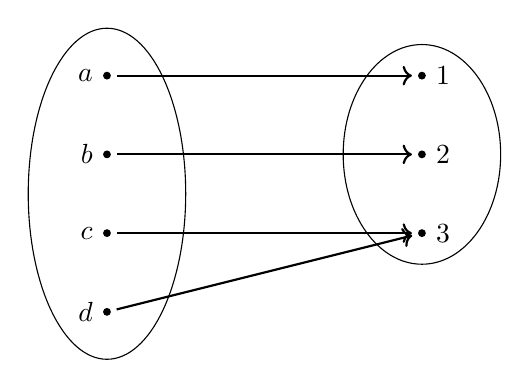
\begin{tikzpicture}[ele/.style={fill=black,circle,minimum width=.8pt,inner sep=1pt},every fit/.style={ellipse,draw,inner sep=-2pt}]
     \node[ele,label=left:$a$] (a1) at (0,4) {};    
     \node[ele,label=left:$b$] (a2) at (0,3) {};    
     \node[ele,label=left:$c$] (a3) at (0,2) {};
     \node[ele,label=left:$d$] (a4) at (0,1) {};
   
     \node[ele,,label=right:$1$] (b1) at (4,4) {};
     \node[ele,,label=right:$2$] (b2) at (4,3) {};
     \node[ele,,label=right:$3$] (b3) at (4,2) {};
   
     \node[draw,fit= (a1) (a2) (a3) (a4),minimum width=2cm] {} ;
     \node[draw,fit= (b1) (b2) (b3), minimum width=2cm] {} ;  
     \draw[->,thick,shorten <=2pt,shorten >=2] (a1) -- (b1);
     \draw[->,thick,shorten <=2pt,shorten >=2] (a2) -- (b2);
     \draw[->,thick,shorten <=2pt,shorten >=2] (a3) -- (b3);
     \draw[->,thick,shorten <=2pt,shorten >=2] (a4) -- (b3);
    \end{tikzpicture}
\end{figure}
Another name for a surjection is an "onto" function because the we are mapping $A$ onto the entirety of $B$.
\begin{definition}
    An injection $f:A\rightarrow B$ is a function where $\forall (x_1, x_2) \in A, ((x_1\ne x_2)\implies f(x_1)\ne f(x_2))$
\end{definition}
\begin{figure}[h]
    \centering
    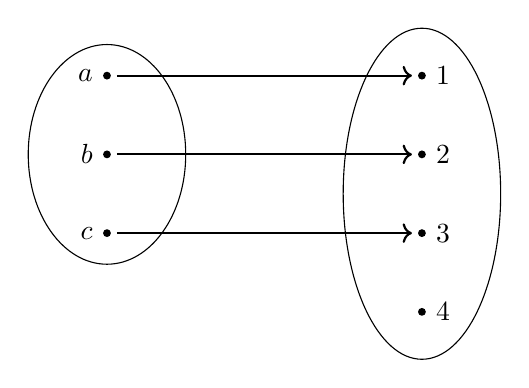
\begin{tikzpicture}[ele/.style={fill=black,circle,minimum width=.8pt,inner sep=1pt},every fit/.style={ellipse,draw,inner sep=-2pt}]
     \node[ele,label=left:$a$] (a1) at (0,4) {};    
     \node[ele,label=left:$b$] (a2) at (0,3) {};    
     \node[ele,label=left:$c$] (a3) at (0,2) {};
   
     \node[ele,,label=right:$1$] (b1) at (4,4) {};
     \node[ele,,label=right:$2$] (b2) at (4,3) {};
     \node[ele,,label=right:$3$] (b3) at (4,2) {};
     \node[ele,,label=right:$4$] (b4) at (4,1) {};
   
     \node[draw,fit= (a1) (a2) (a3),minimum width=2cm] {} ;
     \node[draw,fit= (b1) (b2) (b3) (b4), minimum width=2cm] {} ;  
     \draw[->,thick,shorten <=2pt,shorten >=2] (a1) -- (b1);
     \draw[->,thick,shorten <=2pt,shorten >=2] (a2) -- (b2);
     \draw[->,thick,shorten <=2pt,shorten >=2] (a3) -- (b3);
    \end{tikzpicture}
\end{figure}
In English, this means that every element in the codomain corresponds to at most 1 element in the domain. This is why injections
are also called "one-one" functions. Notice that not all elements in $B$ have to have a corresponding element in $A$.
\begin{definition}
    A function $f:A\rightarrow B$ is a bijection if $f$ is both an injection and a surjection.
\end{definition}
\begin{figure}[h]
    \centering
    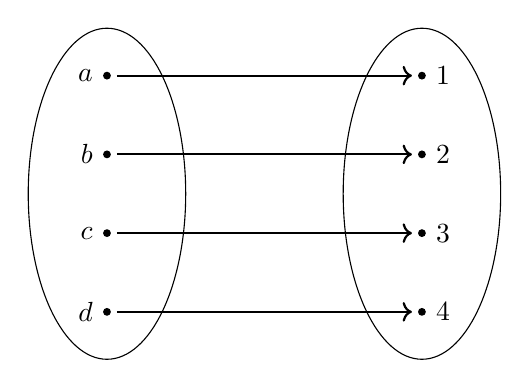
\begin{tikzpicture}[ele/.style={fill=black,circle,minimum width=.8pt,inner sep=1pt},every fit/.style={ellipse,draw,inner sep=-2pt}]
     \node[ele,label=left:$a$] (a1) at (0,4) {};    
     \node[ele,label=left:$b$] (a2) at (0,3) {};    
     \node[ele,label=left:$c$] (a3) at (0,2) {};
     \node[ele,label=left:$d$] (a4) at (0,1) {};
   
     \node[ele,,label=right:$1$] (b1) at (4,4) {};
     \node[ele,,label=right:$2$] (b2) at (4,3) {};
     \node[ele,,label=right:$3$] (b3) at (4,2) {};
     \node[ele,,label=right:$4$] (b4) at (4,1) {};
   
     \node[draw,fit= (a1) (a2) (a3) (a4),minimum width=2cm] {} ;
     \node[draw,fit= (b1) (b2) (b3) (b4), minimum width=2cm] {} ;  
     \draw[->,thick,shorten <=2pt,shorten >=2] (a1) -- (b1);
     \draw[->,thick,shorten <=2pt,shorten >=2] (a2) -- (b2);
     \draw[->,thick,shorten <=2pt,shorten >=2] (a3) -- (b3);
     \draw[->,thick,shorten <=2pt,shorten >=2] (a4) -- (b4);
    \end{tikzpicture}
\end{figure}
Bijections are nice because every element in the codomain is corresponds to a single element in the domain (one-one)
and every element in the codomain is covered by an element in the domain (onto). This gives us an interesting way to 
check if two sets are of equal size. Let's say from sets $X$ and $Y$, we pair up $(x_i, y_i)$. If you can be done no 
elements left over, then the two sets are the same size. If you have elements from either set which are left over 
after pairing the elements up, the sets must be different sizes. Notice that this is the same thing as forming a bijection
between the two sets. This leads us to an important theorem.
\begin{theorem}
    Two sets have the same cardinality if and only if there exists a bijection between them
\end{theorem}
It turns out that sometimes we don't even have to find the actual bijection to prove that two sets have the same cardinality because of the following theorem.
\begin{theorem}
    If there exists an injection $f:A\rightarrow B$ and an injection $g:B\rightarrow A$, then
    there exists a bijection $h:A\rightarrow B$
\end{theorem}
\subsection{Countable Sets}
By using the bijection method of measuring cardinalities, we can "count" sets with an infinite number of elements because all we have to do is
establish a bijection between this set and another set we know is countable. What makes a set countable?
\begin{definition}
    A set $S$ is countable if there exists a bijection $f:S\rightarrow\mathbb{N}$ or some subset of $\mathbb{N}$
\end{definition}
We can think of the natural numbers, a.k.a the counting numbers, as the most fundamental countably infinite set. There are many different
ways which we can construct bijections. One way is to explicitly define the mathematically relationship
which forms the bijection. Another method is to do this pictorally. For example, when checking if $\mathbb{N}\times\mathbb{N}$
is countable, we might draw the following picture:
\begin{figure}[h]
    \centering
    \begin{tikzpicture}
        \matrix(m)[matrix of math nodes,column sep=1cm,row sep=1cm]{
            (0, 3) & \cdots \\
            (0, 2) & (1, 2) & \cdots \\
            (0, 1) & (1, 1) & (2, 1) & \cdots \\
            (0, 0) & (1, 0) & (2, 0) & (3, 0) & \cdots \\
        };
        
        \draw[->]
            (m-4-1)edge(m-4-2)
            (m-4-2)edge(m-3-1)
            (m-3-1)edge(m-2-1)
            (m-2-1)edge(m-3-2)
            (m-3-2)edge(m-4-3)
            (m-4-3)edge(m-4-4)
            (m-4-4)edge(m-3-3)
            (m-3-3)edge(m-2-2)
            (m-2-2)edge(m-1-1);
        \end{tikzpicture}
\end{figure}
Notice that this enumerates all of the possible tuples in $\mathbb{N}\times\mathbb{N}$.
We can also use the theorem presented above where if we can inject $A$ into $B$ and $B$ into $A$, then
then there is bijection between the two sets. This is powerful because we don't actually have to find the bijection.
\subsection{Uncountable Sets}
Just like $\mathbb{N}$ is the "fundamental" countable infinite set, $\mathbb{R}$ is the "fundamental" Uncountable set.
\begin{theorem}
    $\mathbb{R}$ is uncountable, and every interval in $\mathbb{R}$ is uncountable.
\end{theorem}
One way to prove a set is uncountable is to prove a bijection exists to $\mathbb{R}$. However, sometimes this can be quite difficult.
In that case, a proof technique called Cantors Diagonalization can be useful. To see how it works, lets apply it to prove the interval $[0, 1]\in\mathbb{R}$
is uncountable.
\begin{proof}[Cantors Diagonalization]
    We can write $r\in[0, 1]$ as an infinite decimal with no trailing 0s.
    Suppose for contradiction that there exists a bijection from $\mathbb{N}$ to $[0, 1]$.
    This bijection might look as follows:
    \centering
    \begin{tabular}{cccccccc}
        f(0) = 0. & 3 & 7 & 2 & 6 & 5 & 9 & ...\\
        f(1) = 0. & 9 & 9 & 9 & 9 & 9 & 9 & ...\\
        f(2) = 0. & 1 & 0 & 1 & 0 & 1 & 0 & ...\\
        & & & & \vdots
    \end{tabular}
    We can now construct a real number $s\in[0, 1]$ that differs from $f(i)$ in the $ith$ digit $\forall i\in\mathbb{N}$
(a.k.a the diagonal elements). This number must be enumerated by $f(n)$ for $n\in\mathbb{N}$. However, by construction,
$s$ differs from $f(n)$ in the nth digit. This a contradiciton, therefore no such bijection can exist, so the interval is uncountable.
\end{proof}
All diagonalization proofs layout in that same fashion.
\section{Counting}
A very useful skill to have is counting all of the possible ways we can do something. In general, counting problems fall in 4 broad categories.
\begin{itemize}
    \item[1.] Ordered objects, sampling with replacement
    \item[2.] Ordered objects, sampling without replacement
    \item[3.] Unordered objects, sampling with replacement
    \item[4.] Unordered objects, sampling without replacement    
\end{itemize}
When we say "orderered objects" that means ordering matters in the different possibilities. For example, putting $n$ people 
into a line is fundamentally ordered because their position in line matters. When we say sampling with replacement, that means
the same object can show up in one of our possibilities twice. Without replacement means each object in our possibility is distinct.
When we consider how to count each of these scenarios, we use the first and second rules of counting.
\begin{theorem}[First Rule of Counting]
    Suppose an object is formed by a succession of $k$ choices. The total number of distinct objects we can form is
    $\prod_{i=1}^{k}{n_k}$ where $n_k$ is the number of ways the $ith$ choice can happen.
\end{theorem}
\begin{theorem}[Second Rule of Counting]
    Suppose an object is formed by a succesion of $k$ choices, but the order of those choices does not matter.
    The number of possible objects is the number of objects where order doesn't matter divided by the number of ways
    we can rearrage the elements in each object.
    $$\frac{\prod_{i=1}^{k}{n_k}}{k!}$$
\end{theorem}
The first and second rules correspond to counting ordered and unordered objects respectively. Let's see how they can be applied to 4 different
types of counting problems.
\subsection{Ordered Objects, Sampling with replacement}
We can apply the first rule of counting. We are making $k$ choices, and there are $n$ objects to choose from
for each choice we make. This means there are $n^k$ total choices.
\subsection{Ordered Objects, Sampling without replacement}
Once again, we can apply the first rule of counting. We are making $k$ choices. For the first choice, there are $n$ options.
For the second choice, there are $n-1$ options because we can't pick the same element twice. Likewise, for the 3rd choice, we have $n-2$ options.
This gives the product
$$n(n-1)(n-2)...(n-k+1) = \frac{n!}{(n-k)!}$$
\end{document}